\let\negmedspace\undefined
\let\negthickspace\undefined
\documentclass[journal,12pt,twocolumn]{IEEEtran}
\usepackage{cite}
\usepackage{amsmath,amssymb,amsfonts,amsthm}
\usepackage{algorithmic}
\usepackage{graphicx}
\usepackage{textcomp}
\usepackage{xcolor}
\usepackage{txfonts}
\usepackage{listings}
\usepackage{enumitem}
\usepackage{mathtools}
\usepackage{gensymb}
\usepackage{comment}
\usepackage[breaklinks=true]{hyperref}
\usepackage{tkz-euclide} 
\usepackage{listings}
\usepackage{gvv}  
\usepackage{tikz}
\usepackage{circuitikz} 
\usepackage{caption}
\def\inputGnumericTable{}              
\usepackage[latin1]{inputenc}          
\usepackage{color}                    
\usepackage{array}                     
\usepackage{longtable}                 
\usepackage{calc}                     \usepackage{multirow}                  
\usepackage{hhline}                    
\usepackage{ifthen}                    
\usepackage{lscape}
\usepackage{amsmath}
\newtheorem{theorem}{Theorem}[section]
\newtheorem{problem}{Problem}
\newtheorem{proposition}{Proposition}[section]
\newtheorem{lemma}{Lemma}[section]
\newtheorem{corollary}[theorem]{Corollary}
\newtheorem{example}{Example}[section]
\newtheorem{definition}[problem]{Definition}
\newcommand{\BEQA}{\begin{eqnarray}}
\newcommand{\EEQA}{\end{eqnarray}}
\newcommand{\define}{\stackrel{\triangle}{=}}
\theoremstyle{remark}
\newtheorem{rem}{Remark}

%\bibliographystyle{ieeetr}
\begin{document}
%

\bibliographystyle{IEEEtran}




\title{
%	\logo{
G.A.T.E.

\large{EE1205 : Signals and Systems}

Indian Institute of Technology Hyderabad
%	}
}
\author{Chirag Garg

(EE23BTECH11206)
}	





\maketitle

\newpage



\bigskip

\renewcommand{\thefigure}{\theenumi}
\renewcommand{\thetable}{\theenumi}


\section{Question E.C.(45)}
\vspace{0.5cm}



\textbf{Question:} Let a frequency modulated (FM) signal : $ x(t) = A \cos(\omega_c t + k_f \int_{-\infty}^{t} m(\lambda) d\lambda)$ , where $ m(t) $is a message signal of bandwidth $ W $. It is passed through a non-linear system with output $y(t) = 2x(t) + 5(x(t))^2 $.
Let $B_T $ denote the FM bandwidth. The minimum value of $ \omega_c $ required to recover $ x(t) $ from $ y(t) $ is:\\
\begin{enumerate}[label = (\Alph*)]
\item $B_T + W$ \\
\item $\dfrac{3}{2} B_T$ \\
\item $2B_T + W$ \\
\item $\dfrac{5}{2} B_T$ \\
\end{enumerate} \hfill{(GATE EC 2023)}\\
%\section{Solution} 
\textbf{Solution: }
\begin{table}[h!]
\centering
\resizebox{\columnwidth}{!}{
\begin{tabular}{|c|c|c|}
    \hline
     \textbf{Parameter} & \textbf{Value} &
     \textbf{Description}\\
    \hline 
     $\phi(t)$ &  $k_f \int_{-\infty}^{t} m(\lambda) d\lambda$ & Phase\\
    \hline 
     $x(t)$ &  $A \cos(\omega_c t + \phi(t))$ & FM Signal\\
     
    \hline
     $y(t)$ & $2x(t) + 5(x(t))^2 $ & Output from system  \\
      \hline
      
    
  
								      
\end{tabular}}
\label{cggattab1}
\caption*{ TABLE 1:Given Parameters}
\end{table}
\\
\begin{align}
BW[x(t)] \longrightarrow B_T = 2(\omega + \triangle f )
\end{align}
\begin{figure}[h!]
  \centering
  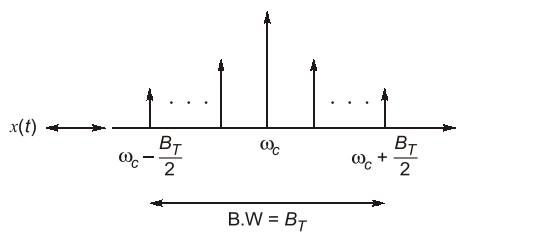
\includegraphics[width=0.5\textwidth]{figures/cggatefig1.png} 
 \label{cggatefig1}
 \caption*{Fig. 1}
\end{figure}

Now , for $x^{2}(t) $
\begin{align}
\triangle f' = 2\triangle f \\
\omega'_C = 2\omega_C
\end{align}

\begin{figure}[h!]
  \centering
  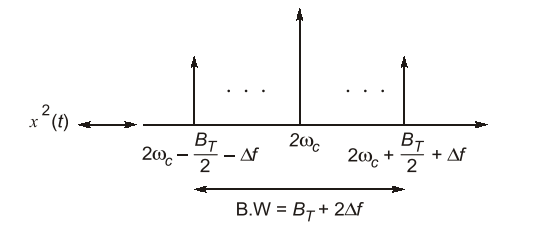
\includegraphics[width=0.5\textwidth]{figures/cggatefig2.png} 
 \label{cggatefig2}
  \caption*{Fig. 2}
\end{figure}

\begin{align}
BW[x^2(t)] &= 2(\triangle f' + \omega) \\
&=2(2\triangle f + \omega) \\
&=B_T + 2\triangle f
\end{align}

\begin{align}
y(t) = 2x(t) + 5(x(t))^2
\end{align}

\begin{figure}[h!]
  \centering
  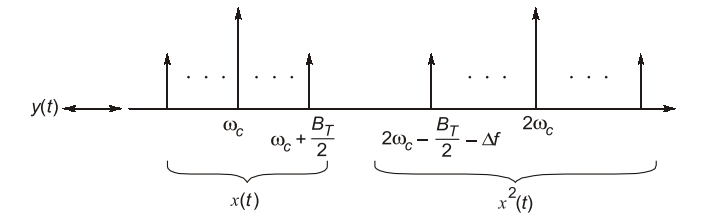
\includegraphics[width=0.5\textwidth]{figures/cggatefig3.png} 
 \label{cggatefig3}
  \caption*{Fig. 3}
\end{figure}

To recover $x(t)$ ,
\begin{align}
2\omega_C - \dfrac{B_T}{2} - \triangle f > \omega_C + \dfrac{B_T}{2} \\
\omega_C > \triangle f + B_T \\
\omega_C > \triangle f + 2(\omega + \triangle f) \\
\omega_C > 3\triangle f + 2\omega \\
\omega_C > \dfrac{3}{2}[2(\triangle f + \omega)] - \omega \\
 \omega_C > \dfrac{3}{2}B_T - \omega
\end{align}

\begin{align}
\therefore (\omega_C)_{min} = \dfrac{3}{2}B_T
\end{align}

Hence the correct option is $(b)$
\end{document}